%!TEX root = main.tex
\documentclass[main.tex]{subfiles}

\begin{document}

\chapter{Speech processing using pre-trained models}

\vspace{3em}

\corr{As outlined at the end of the previous chapter (§\ref{sec:published}), the work presented in this dissertation has been published or accepted for publication at the time of writing (March 2024), with some appearing several years earlier \parencite[e.g.][]{san2021leveraging}.~That is, some areas have seen even more recent developments following the work presented.~The goal of this chapter is thus twofold: to not only provide the background on speech processing and recently developed pre-trained models to understand content contained in this dissertation, but also situate the content in relation to related work current at the time of writing.~Additionally, to cater to multiple audiences and interests, from the documentarian wanting a broad overview of speech processing to a computational linguist wanting to build on this body of work, this chapter is divided into three parts, each increasing in the level of technical detail.~In the first part (§\ref{sec:speech-intro}), I provide a high-level introduction to speech processing and various technical terms used in the remainder of this dissertation.~In the second part (§\ref{sec:chp2-w2v2}), I provide a mixed-level overview of wav2vec 2.0 (a framework for developing pre-trained models for speech processing), where occasional low-level details are provided as footnotes to relatively high-level text.~In explicit terms: the start and ends of each paragraph in this section provide high-level explanations along with narrative scaffolding, though lower-level details may also be present in the middle of some.~Finally, in the third part (§\ref{sec:speech-related}), I provide a synthesis of related work where I assume some familiarity with the lower-level details of various models and methods.~The remainder of the dissertation may be understood without reading this section.}

\section{An introduction to speech processing}
\label{sec:speech-intro}

\begin{figure}[!ht]
  \centering
  \vspace{2em}
  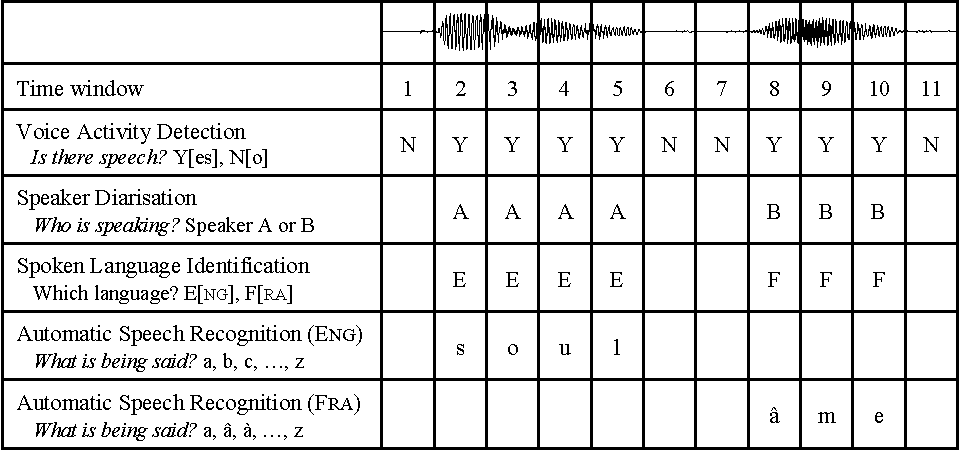
\includegraphics[width=0.85\linewidth]{figures/intro-speech-tasks}
  \caption[A high-level illustration of various speech processing tasks]{A high-level illustration of various speech processing tasks, illustrated using an English (E{\footnotesize{}NG}) speaker eliciting a word of interest from a speaker of French (F{\footnotesize{}RA}).}
  \label{fig:intro-speech-tasks}
\end{figure}


\subsection{Speech processing tasks}

\corr{The various tasks found in the speech processing literature can be understood as processes that help annotate speech with specific information}.~Figure \ref{fig:intro-speech-tasks} provides a summary of common speech processing tasks, illustrated using an excerpt of speech where an English speaker is eliciting from a French speaker some word of interest, \emph{âme} `soul'.~At a high-level, each of these tasks can be understood as training a model to predict the answer to a multiple-choice question for a given time window of speech.~Each task differs from the others in the question under consideration and in the possible answers,~e.g.~Voice Activity Detection (VAD): \emph{Is there speech?}~Yes/No.~Despite these differences, all tasks have a common need to extract relevant information from the speech signal.~In other words, all tasks stand to benefit from an adaptable, general-purpose model that can assist in this common sub-task of information extraction.

\subsection{Speech processing using pre-trained models}
\label{sec:chp2-FMs}

An emerging class of models for building artificial intelligence (AI) systems is foundation models \parencite[FMs:][]{bommasani2021opportunities}, also known as `general-purpose' or `base' or `pre-trained' models.\footnote{Given its widespread use in the speech processing domain, I adopt the term pre-trained models throughout this dissertation.}~Across many domains, these models have led to a paradigm shift in AI system development.~As illustrated in Figure \ref{fig:intro-conv-vs-fm}, this paradigm consists of a pre-training stage where a model is first trained on unlabelled data using a proxy task which permits the resulting pre-trained model to be re-used for various target tasks at a later stage.~A common proxy task for pre-training is masked modelling where, as illustrated in Figure \ref{fig:intro-conv-vs-fm} (i), the model is given a partially masked input and is then tasked with using the neighbouring, unmasked regions to predict the contents of the masked ones.~As labels for this proxy task can be derived automatically without the need for humans (i.e.~it is `self-supervised'), the pre-training stage can leverage substantially larger amounts of data than previously possible (e.g.~half a million hours of untranscribed speech).~This large-scale pre-training is commonly considered a key ingredient for the adaptability of these models for various downstream tasks even with only limited task-specific data \parencite[][]{bommasani2021opportunities}.

\begin{figure}[H]
  \centering
  \vspace{1em}
  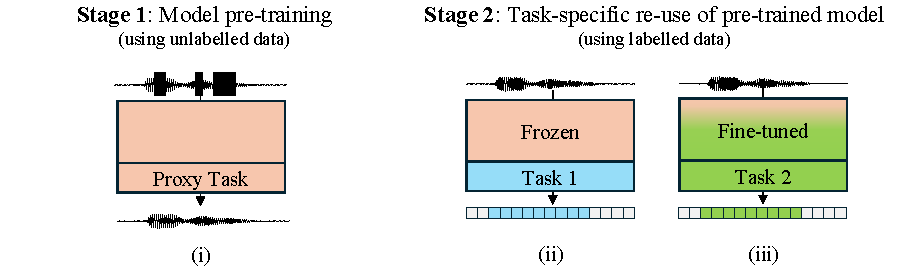
\includegraphics[width=0.85\linewidth]{figures/intro-pt-paradigm}

  \caption[System development paradigm based on pre-trained models]{System development paradigm based on pre-trained models.}
  \label{fig:intro-conv-vs-fm}
\end{figure}

Given a pre-trained model, it may be re-used for target tasks in several ways.~For relatively straightforward classification tasks (e.g.~spoken language identification, spoken term detection), the information extracted from the input by the pre-trained model (or its `representations') may be sufficient to use as-is.~In these cases where the model is not further trained, or used `frozen' as illustrated in Figure \ref{fig:intro-conv-vs-fm} (ii), its representations are simply fed into another model which is trained to predict the task-specific labels based on these representations.~For more complex text-generation tasks (e.g.~ASR), the model may need to be adapted for the target task through further training, or `fine-tuning' as illustrated in Figure \ref{fig:intro-conv-vs-fm} (iii).~In these cases, both the pre-trained and task-specific models are trained together to predict the task-specific labels.~Additionally, if the data on which the model was pre-trained is significantly different from the data to be used in the target task, the pre-trained model can also be adapted via `continued pre-training' \parencite[CPT:][]{gururangan2020don} using all available unlabelled target data (e.g.~untranscribed audio), only after which this adapted model is fine-tuned with the more limited labelled subset (e.g.~audio paired with human transcriptions for ASR).

\section{wav2vec 2.0: A framework for pre-training models for speech processing}
\label{sec:chp2-w2v2}

\corr{In this section, I provide a detailed introduction to wav2vec 2.0, a framework for developing pre-trained models for speech processing that has seen widespread proliferation.~As mentioned above, self-supervised pre-training has enabled models to be trained without requiring any human labels and consequently at increasingly larger scales}.~Since the release of the original English model pre-trained on 960 hours of English \parencite{NEURIPS2020_92d1e1eb}, there have been additional larger-scale variants both domain-specific and multilingual, one or more of which were used for experiments presented in Chapters 3--6.~For example, the Robust variant \parencite{hsu2021robust}, intended for noisy speech domains, is pre-trained on 63k hours of English speech (including audio from noisy telephone conversations).~Multilingual variants include XLSR-53, pre-trained on 56k hours from 53 languages \parencite{conneau21_interspeech}; XLSR-128, pre-trained on 436k hours from 128 languages \parencite{babu22_interspeech}; and MMS, pre-trained on 491k hours from 1,406 languages \parencite{pratap2023scaling}.

\corr{At a high-level, the wav2vec 2.0 model architecture and pre-training process can be thought of as tasking the model to discover --- based on raw audio alone --- a useful set of discrete units (e.g.~\{\emph{a, b, ..., z}\}) with which it is able to carry out a speech variant of a Cloze test:~e.g. given ``\textit{The big \_ \_ \_ chased the small rat.}'', correctly guess for each masked position \emph{c}, \emph{a}, and \emph{t}, respectively}.~Accordingly, as illustrated in Figure~\ref{fig:w2v2-chp2}, the wav2vec 2.0 architecture consists of three parts:~1) a convolutional feature extractor that extracts learnable features from strided frames in the audio input,~2) a quantiser which clusters the audio features into a set of discrete code vectors ($q_1$, ..., $q_5$),~and 3) a transformer attention network that learns context-enriched representations ($h_1$, ..., $h_5$).~For self-supervised pre-training, the model is optimised using a joint contrastive loss and a diversity loss.~The contrastive loss requires the model to use the neighbouring context to distinguish masked frames amongst a set of negative distractors.~The diversity loss requires the model to make equal use of all code vectors, preventing the model from relying on a small subset which can lead to trivial/sub-optimal solutions.

\begin{figure}[H]
    % \vspace{-0.5em}
    \centering
    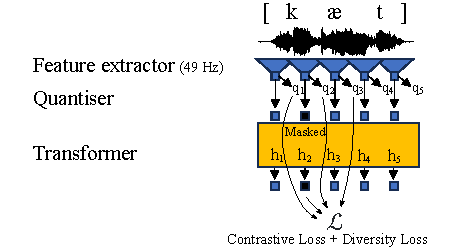
\includegraphics[width=0.50\linewidth]{figures/sigtyp2024-w2v2-v2}
    \caption[Illustration of the wav2vec 2.0 architecture]{Illustration of the wav2vec 2.0 architecture. Adapted from \textcite{NEURIPS2020_92d1e1eb}.}
    % \vspace{-0.5em}
    \label{fig:w2v2-chp2}
\end{figure}

\corr{One consequence of the wav2vec 2.0 model architecture and pre-training objectives is that the representations learned through pre-training are relatively fine-grained.~For example, as illustrated in Figure \ref{fig:w2v2-chp2}, a single speech sound such as [\ae] may last for three time steps (yielding three code vectors: $q_2, q_3, q_4$), since the model encodes speech at a rate of of 49 Hz.~When combined with the diversity loss that requires the model to equally make use of all code vectors, this results in a complex many-to-many mapping between the learned discrete codes and more coarser linguistic units such as phones.}

\subsection{Probing wav2vec 2.0 representations}
\label{sec:w2v2-probing}

\corr{One active area of research is in understanding what kinds of information are learned at the various stages in the models \parencite[e.g.][]{ma2021probing,bartelds2022neural,pasad2021layer,pasad2023comparative,pasad2024self,abdullah2023information}.~One finding from this body of work is that, while the mapping between them is complex, the discrete codes do consistently correspond to a specific of speech sound, or a set thereof.~For example, as illustrated in Figure \ref{fig:abdullah2023information}, each discrete code listed with an arbitrary alphanumeric label on the x-axis (e.g.~A46, A29, ..., B1) is typically associated with a small set of phones (e.g.~A46 with velar stops [k] and [g]).}

\begin{figure}[H]
    % \vspace{-0.5em}
    \centering
    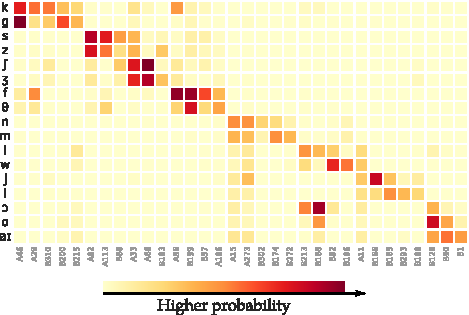
\includegraphics[width=0.65\linewidth]{figures/abdullah2023information-fig1}
    \vspace{-0.5em}
    \caption[Probability of English phone categories for a given discrete unit learned by the wav2vec 2.0 XLSR-53 model]{\corr{Probability of English phone categories for a given discrete unit learned by the wav2vec 2.0 XLSR-53 model.~Figure sourced from \textcite{abdullah2023information}, used with permission from Badr Abdullah.}}
    % \vspace{-0.5em}
    \label{fig:abdullah2023information}
    % \vspace{-0.5em}
    \centering
    
    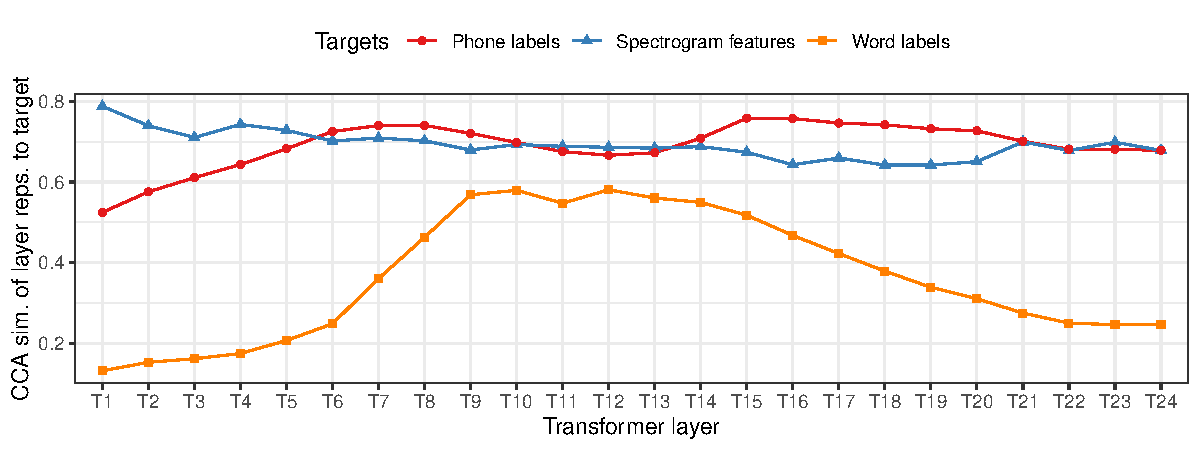
\includegraphics[width=1\linewidth]{figures/pasad2023w2v2-lv60}
    \vspace{-2.5em}
    \caption[Similarity of transformer layer outputs to spectrogram features, phone labels, and word labels]{\corr{Similarity of transformer layer outputs to spectrogram features, phone labels, and word labels.~Similarities calculated using canonical correlation analysis (CCA) on English using the wav2vec 2.0 LV-60 model, reported in \textcite{pasad2023comparative}.~Figure re-produced using data provided by Ankita Pasad.}}
    \label{fig:pasad2023w2v2-lv60}
\end{figure}

\corr{Another finding is that the type and degree of linguistic information contained in the model's intermediate representations varies from layer to layer.~For example, as illustrated in Figure \ref{fig:pasad2023w2v2-lv60}, the representations of the very first transformer layer (T1) is highly similar to those extractable using conventional spectrograms and this similarity decreases in later layers.~Similarly, linguistic information related to word identity is found in the middle layers (e.g.~T12) while information related to phone identity in later ones (e.g.~T16).~Investigating what information is learned in which layers and why is an active area of research, only briefly noted here.~For our interest in using wav2vec 2.0 models for various speech tasks, we simply note that certain tasks may benefit more from using a middle layer while others benefit from later ones.}

\corr{As mentioned above, a pre-trained model such as wav2vec 2.0 may be used `frozen' (i.e.~without additional training to simply help extract speech information) or `fine-tuned' (i.e.~with additional training using task-specific labels such as transcriptions for the ASR task).~In the remainder of this subsection, I detail the use of wav2vec 2.0 models in each of these two configurations through two relevant tasks: spoken term detection and automatic speech recognition.}

\subsection{Using frozen wav2vec 2.0 representations for spoken term detection}

\corr{In the task of spoken term detection, we are interested in determining whether a given spoken query occurs within some other spoken utterance, known as the `test item'.~Given that a query may be spoken by one person in one recording environment (e.g.~a loud, high-pitched speaker in a quiet room) while the test item may be spoken by another person in a different one (e.g.~a quiet, low-pitched speaker in noisy room), a critical part of successfully carrying out this audio-on-audio comparison is obtaining a speaker-invariant and noise-robust representation of the phonetic content in the query and test item.}

\begin{figure}[H]
  \centering
  \vspace{1em}
  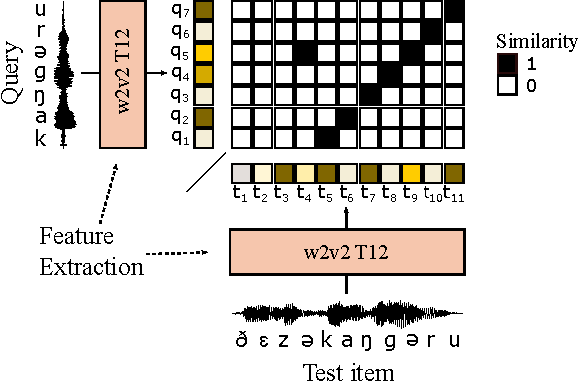
\includegraphics[width=0.60\linewidth]{figures/asru2021-qbestd-stages-w2v2}
  \caption[Using transformer representations from a wav2vec 2.0 model as a features for the spoken term detection task]{Using transformer representations from a wav2vec 2.0 model as a features for the spoken term detection task.}
  \label{fig:chp2-qbestd-feat}
\end{figure}

\corr{The use of a wav2vec 2.0 model as a feature extractor for spoken term detection is illustrated in Figure~\ref{fig:w2v2-chp2}.~In this example, we have a query \emph{kangaroo} [{\fontspec{LinLibertine.ttf}kaŋgəru}] and test item \emph{there’s a \underline{kangaroo}} [{\fontspec{LinLibertine.ttf}ðɛzəkaŋgəru}], and are interested in correctly detecting that the query does indeed occur within the test item.~To carry out this task, we first derive speech representations extracted from the 12th transformer layer of a wav2vec 2.0 model, which we will see in Chapter 3 is consistently the most well suited layer for this task.~This feature extraction process yields for the query a sequence of vectors $q_1, ..., q_7$ each representing the speech content at some given time window in the query.~Similarly, we use the same process to derive a corresponding sequence for the test item, $t_1, ..., t_{11}$.

These vectors can then be used by a spoken term detection model which compares the similarity of each pair of vectors (e.g. $q_1$ vs. $t_1$, ..., $q_7$ vs. $t_{11}$) and returns a score of how likely the query is to be found within the test item.~For example, $q_1$ vs. $t_1$ has a similarity of 0, given the [k]-initial query \emph{\textbf{k}angaroo} vs. the [{\fontspec{LinLibertine.ttf}ð}]-initial test item \emph{\textbf{th}ere's a kangaroo}.~By contrast, $q_7$ vs. $t_{11}$ has a similarity of 1 as both end in the same vowel [u].~Conventionally, this detection stage is typically carried using using some form of Dynamic Time Warping (DTW) based algorithm, though we review more recent alternatives in the related work section of this chapter.~Roughly summarised, the task of this model is to use the representations to look for whether there is a highly correlated region between the query and test item, as illustrated by the diagonal in Figure~\ref{fig:chp2-qbestd-feat}.}

\subsection{Fine-tuning wav2vec 2.0 models for automatic speech recognition}
\label{sec:w2v2-decoding}

\corr{As mentioned, in more complex text generation tasks such as ASR, the wav2vec 2.0 model is typically further trained or `fine-tuned' for this target task.~This is typically done by appending another model,\footnote{This `model' may be as simple as a linear layer or as complex as a pre-trained decoder-only text transformer model.} after which both models are jointly optimised for the ASR task.\footnote{Typically using a loss such as Connectionist Temporal Classification \parencite[CTC:][]{graves2006connectionist}.}~Similar to the frozen use, this process amounts to using the pre-trained wav2vec 2.0 model to encode the speech into some intermediate set of representations from which a decoding process uses those representations to generate a sequence of characters, e.g. \emph{too dogz} as illustrated in Figure \ref{fig:chp2-w2v2-asr}.~In contrast to the frozen use case,\footnote{Though note however the wav2vec 2.0 encoder is typically frozen for the first 10k steps when starting with a randomly-initialised linear layer \parencite[][§4.3]{NEURIPS2020_92d1e1eb}} the fine-tuning process adjusts the wav2vec 2.0 model to better extract representations optimised for this new text generation task.}

\begin{figure}[H]
  \centering
  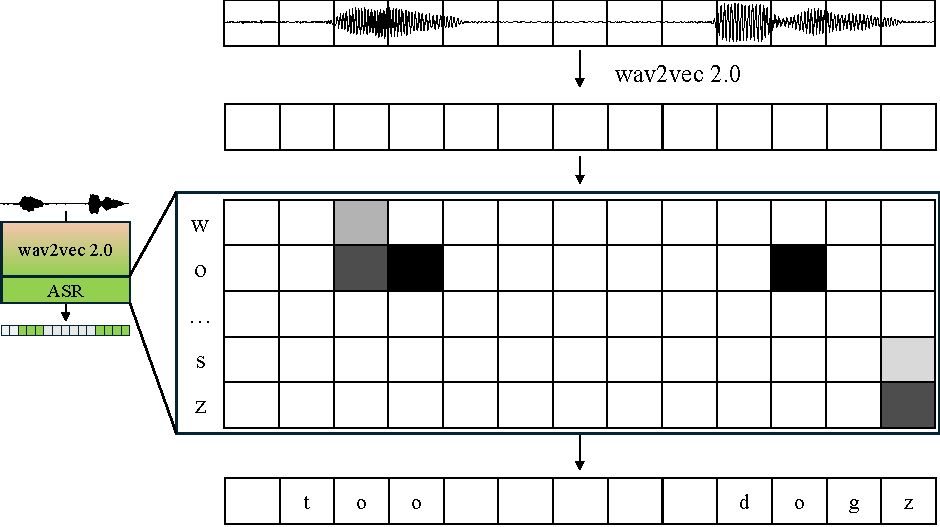
\includegraphics[width=0.85\linewidth]{figures/w2v2-asr-ft}
  \caption{\corr{Fine-tuning a wav2vec 2.0 model for the automatic speech recognition task}}
  \label{fig:chp2-w2v2-asr}
\end{figure}

\corr{As seen in this transcription \emph{too dogz}, the generated transcriptions from a wav2vec 2.0 model fine-tuned for ASR with only limited transcriptions may be rather error prone, as the system has seen very few pairs of sound and character sequences to learn from.~For machine-assisted transcription to be viable (and save human effort), it is desirable for the machine-generated transcriptions to contain as few errors as possible --- a transcription that is entirely incorrect may even take longer to correct than manual transcription.~In Chapters 4 and 5, we examine how transcription errors can be reduced using assistive processes.}

\corr{First, an `unassisted' decoding process that is most commonly used is in the ASR literature is known as greedy decoding.~As illustrated in Figure \ref{fig:chp2-w2v2-asr}, part of the ASR process involves determining a single character for each output time step based on a probability distribution over the character set at each time step.\footnote{In some cases, it may be a set of sub-word units, see \textcite[][§3.2]{ahmed2023improving} and works cited therein.~This, however, typically assumes there is text data on which a good sub-word model can be trained and sufficient transcriptions for fine-tuning to learn mappings to a larger vocabulary size (e.g. 256 sub-word units vs. 27 characters).}~For example, at the third time step, while both \emph{w} (light grey) and \emph{o} (dark grey) are noted as probable at this time step, the latter has been predicted as being more likely.~A similar split is found between, \emph{s} and \emph{z} in the last time step.~In greedy decoding, the most probable character is selected as the prediction for each time step --- yielding the prediction \emph{too dogz}.}

\corr{The decoding process may be assisted in two ways when text data is available from sources such as books or the internet.~Using these sources, we can derive a lexicon which contains the various unique words that are possible in the language or additionally train a language model (LM) which observes which word sequences are more probable than others.~Thus, a lexicon- and/or LM-assisted decoding process can limit the ASR system output to only possible words, e.g. \emph{too dogz} $\rightarrow$ \emph{too dogs} as well as bias the output to more probable word sequences, e.g. \emph{too dogs} $\rightarrow$ \emph{two dogs}.~Of course, this assistive process requires that there be external text data and, importantly, the sentences be similar to those in the audio to be transcribed to avoid erroneous miscorrections.~Thus, given enough transcribed speech for ASR fine-tuning, greedy decoding as good as LM-assisted decoding \parencite{synnaeve2019end}.}

\section{Related work}
\label{sec:speech-related}

\subsection{Spoken term detection and open vocabulary keyword spotting}

\corr{As mentioned, the detection stage in spoken term detection has conventionally been implemented using some form of Dynamic Time Warping (DTW) based algorithm.\footnote{For a comprehensive book-length survey of the field, see \textcite{marySearchingSpeechDatabases2018}.}~More recently, there have been both neural and end-to-end approaches proposed.~For example, given that this detection stage lends itself to being reformulated as a computer vision problem (i.e.~detect presence of a diagonal in a 2D matrix), \textcite{ramCNNBasedQuery2018} proposes replacing the DTW-based model with one based on a Convolutional Neural Network (CNN), adopting based on the computer vision literature a VGG-like model \parencite{simonyan2014very}.~In later work, \textcite{ramNeuralNetworkBased2020} propose a fully end-to-end approach without the need for a separate feature extraction stage. }

\corr{What is worth noting, however, is that, at least in this later study \parencite{ramNeuralNetworkBased2020}, the conventional two-stage system with DTW-based classification was the best performing system compared to the CNN and end-to-end ones for lower resource languages in the standard SWS2013 benchmark dataset for spoken term detection.~In other words, the conventional DTW-based approach remains highly competitive when there is insufficient task-specific data for training the classifier model.~To the best of my knowledge, SWS2013 and its successor QUESST2014 (which has fewer low-resource languages), remain the most current spoken term detection benchmarks.\footnote{The annual MediaEval challenge which developed SWS2013 and QUESST2014 has not since featured spoken term detection again as a shared task, see \url{https://multimediaeval.github.io/}.}}

\corr{An alternative, promising starting point that could be drawn upon in future work is the keyword spotting literature, which has seen a recent interest in more open query sets.~Conventionally speaking, spoken term detection is defined as a task with an open query set while its counter-part keyword search or keyword spotting is one with a limited, closed query set.~Nevertheless, the open vocabulary use case is often anticipated and system evaluations may even report out-of-vocabulary performance and performance after few-shot learning on new keywords \parencite[e.g.][]{mazumder2021few,kao2023efficiency,jung2023metric}.~One particularly interesting work in this area is \textcite{zhu2023open}, which both proposes a method for open vocabulary keyword search and releases an associated dataset with more than 115 languages, including 44 based on language documentation projects sourced from DoReCo.\footnote{\url{https://doreco.info/}}}

\subsection{English HuBERT, WavLM, data2vec (2.0) and multilingual w2v-BERT 2.0}

\corr{Since the development of wav2vec 2.0 framework by \textcite{NEURIPS2020_92d1e1eb}, there have been numerous proposals for further improving the speech pre-training process, the most directly related of which I summarise here.~As introduced above, the wav2vec 2.0 pre-training process involves simultaneously learning a set of discrete units and learning to perform a masked prediction task using those units.~By contrast, in HuBERT \parencite{hsu2021hubert}, pre-training process alternates between an acoustic unit discovery stage and the masked prediction stage, whereby acoustic units are iteratively derived from a middle transformer layer of the model trained in the previous iteration (or MFCCs for the very first iteration).~Further modifying the HuBERT pre-training process, WavLM \parencite{chen2022wavlm} proposes data augmentation along with an additional denoising objective in order to optimise representations for tasks beyond ASR (e.g.~speaker verification and identification).~The focus of data2vec and its successor data2vec 2.0 \parencite{baevski2022data2vec,baevski2023efficient} is to derive an efficient pre-training process for multiple modalities: vision, speech, and text.~In contrast to alternating between two stages as in HuBERT/WavLM, the pre-training process leverages a teacher model that is given the whole, unmasked input and whose weights track an exponential moving average of a student model that is given a masked input and is tasked with predicting the representations of the teacher model.~Compared to the 150h of compute time on 64 A100 GPUs required for pre-training the wav2vec 2.0 model, the data2vec 2.0 model for speech required only 76.7h on the same hardware while also performing better when subsequently fine-tuned for English ASR.~All these models from HuBERT to data2vec 2.0, however, are pre-trained only on English.

As mentioned, the last multilingual variant of wav2vec 2.0 is MMS, pre-trained on 491k hours of speech from 1,406 languages \parencite{pratap2023scaling}.~At the time of writing in March 2024, the latest openly available, multilingual model is w2v-BERT 2.0,\footnote{https://huggingface.co/facebook/w2v-bert-2.0} pre-trained on 4.5M hours released in late 2023 as part of a suite of models by \textcite[][see §3.2.1]{barrault2023seamless}.~The notable architecture changes in this model is the use of a joint contrastive loss (similar to wav2vec 2.0, without the diversity loss) and masked prediction loss (similar to HuBERT) though without alternating between two stages (unlike HuBERT), and the use of conventional filterbank features instead of a convolutional feature extractor.\footnote{See \textcite{parcollet23_interspeech} for wav2vec 2.0 pre-training experiments with different feature extraction methods showing minimal degradation in downstream ASR performance, especially considering the compute cost.}~Additionally, in place of a 24-layer transformer network is an equivalent one composed of conformer layers \parencite{gulati2020conformer}, which leverage convolution neural networks to better model local features and complement transformer layers that model the global context.}

\end{document}
